\chapter{Einführung}
\label{sec:intro}
	%\setcounter{page}{1}
	
	Im Laufe der Zeit steigen innerhalb der Industrie die Ansprüche an Qualität und der Identifikation/Dokumentation von Produkten. In diesem Bezug gewinnt die Bildverarbeitung zunehmend an Bedeutung und ist in der automatisierten Produktion heute unabdingbar \cite[S. 1]{indust-imgproc}. 
	Vor allem spielt sie bei der Identifikation eine unverzichtbare Rolle. Dort wird sie zur maschinellen Erfassung optischer Kennzeichnungen, wie sie beispielsweise in Abbildung \ref{fig:example-code} zu sehen sind, eingesetzt:
	\begin{figure}[h]
		\centering
		\subfloat[][Bauteil mit gelasertem Code]{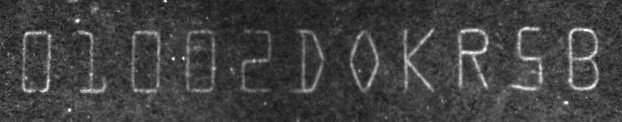
\includegraphics[width=0.48\linewidth]{IMG_01002DOKR5B_c}}
		\qquad
		\subfloat[][Bauteil mit graviertem Code]{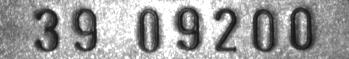
\includegraphics[width=0.48\linewidth]{IMG_3909200}}
		\caption{Beispiel-Bauteile mit unterschiedlichen Einbringungsmethoden für Zeichencodes}
		\label{fig:example-code}
	\end{figure}
	Derartige Codes zu lesen, ist für den Menschen eine triviale Aufgabe, doch für die Maschine bisweilen eines der anspruchsvollsten Probleme in der industriellen Bildverarbeitung. Dabei ist ein essenzieller Arbeitsschritt die Segmentierung der Bilder \cite[S. 136]{indust-imgproc}. Auf der Suche nach einer zufriedenstellenden Lösung müssen unter anderem durch 
	Experimente mit unterschiedlichen Methoden Erkenntnisse gewonnen werden. 
	Hierzu soll im Übrigen auch diese vorliegende Arbeit einen Beitrag leisten, 
	indem sie untersucht, inwieweit ein ausgewähltes Verfahren aus der Gruppe 
	der \textit{evolutionären Methoden} dafür geeignet ist, einen wichtigen 
	Schritt innerhalb der \gls{ocr} zu realisieren. \\
	
	Dabei ist die folgende Struktur vorgesehen: \\
	In Kapitel \ref{sec:prob} werden die Hintergründe bzw. die grundlegende 
	Motivation aus der Bildverarbeitung - spezifischer ausgedrückt, aus der 
	\gls{ocr} - hinter dieser Arbeit beleuchtet.\\
	Kapitel \ref{sec:sol} formuliert konkret die Aufgabenstellung und zeigt Ansätze 
	zur Lösung dieser sowie die Umsetzung in Form von Programmcode auf.\\
	Daraufhin werden in Kapitel \ref{sec:results} die Ergebnisse aus der 
	Umsetzung der in Kapitel \ref{sec:sol} vorgestellten Ideen und eine 
	Interpretation der Resultate präsentiert.\\
	Abgerundet wird dieses Erzeugnis durch eine abschließende Bewertung sowie einen Ausblick auf die künftige Verwendung der in Kapitel \ref{sec:sol} erarbeiteten Implementierung.
